\documentclass[Results.tex]{subfiles} 

\begin{document}

\chapter{Results}

There were 28 replies on the post-questionnaires, two subjects did not reply and are not considered in the study. One of the participants had an extreme anxiety for space-environments, the participant is therefore neither considered in the study. Besides that, for two participants there were hearing problems during one environment (once roller coaster, once space), therefore the ratings of the environment in these cases are not considered.  

\section{Analysis of results}
For the analysis of the results the program IBM SPSS Statistics v20 is used. A significance level $\alpha$ of 0.05 will be held and significances of difference will be tested with the independent samples T Test.

\subsection{Space environment}
To test the correlation between the sounds the participants were exposed to and their rating of the space environment, two plots for the space environment are shown below. In figure \ref{fig:Ratings_sound_BM}, the variables in equal order are the ratings of the participants about: 
\begin{itemize}
	\item How boring it was;
	\item How exciting it was;
	\item How scary it was.
\end{itemize}

\begin{figure}[H]
	\centering
		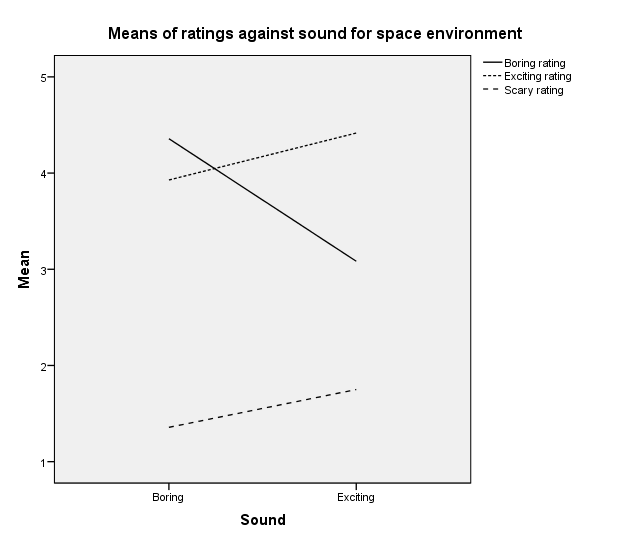
\includegraphics[width=0.90\textwidth]{Section_1/Figures/Ratings_sound_BM.png}
	\caption{Means of the ratings against the sentences the participant heard for the space environment}
	\label{fig:Ratings_sound_BM}
\end{figure}

From the figure we can conclude that the rating of scary was not significantly affected (t(24)=-.872, p=.392) by the boring (M=1.36, SD=1.082) or exciting (M= 1.75, SD=1.215) sentences. For the exciting rating this is neither a significant (t(24)=-698, p=.492) difference for boring sentences (M=3.93, SD=1.592) and exciting sentences (M=4.42, SD=1.975). The rating of boring seems however to be more influenced, however the difference is also not significant (t(24) = 1.951, p= .063) between hearing the boring sentences (M= 4.36, SD=1.692) and the exciting sentences (M=3.08, SD=1.621). \\

The differences of the other ratings of the space environment are shown in figure \ref{fig:Ratings2_sound_BM}. The variables shown in the figure are respectively the ratings of the participants on:
\begin{itemize}
\item How dominant they felt during the experience;
\item How they rated their valence during the experience;
\item How much they would recommend others to do the experience;
\item How much they would like to do the experience again;
\item How they rated their arousal during the experience;
\item How they rated how much fun the experience was;
\item How they rated the impact the experience had two hours after the experience.
\end{itemize}

\begin{figure}[H]
	\centering
		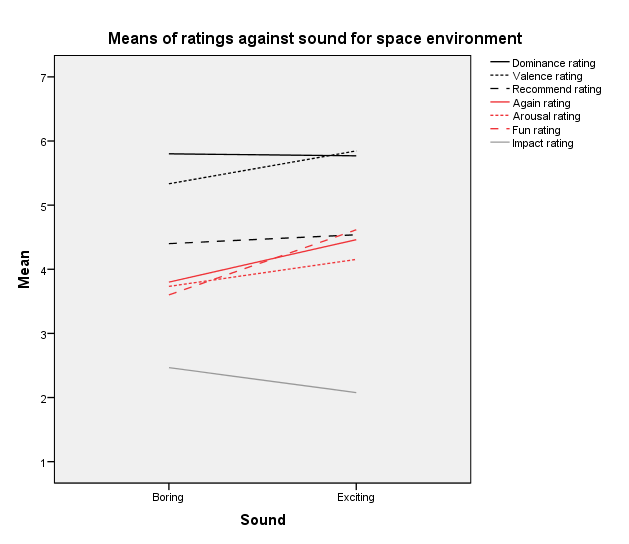
\includegraphics[width=0.90\textwidth]{Section_1/Figures/Ratings2_sound_BM.png}
	\caption{Means of the other ratings against the sentences the participant heard for the space environment}
	\label{fig:Ratings2_sound_BM}
\end{figure}

The rating of fun seems to have a big difference after hearing the boring sentences (M=3.71, SD = 1.59) and the exciting sentences (M=4.67, SD = 1.497) however this difference is not significant (t(24) = -1.564, p=.131). The other differences of ratings are less significant.

\subsection{Roller coaster}
To test the correlation between the sounds the participants were exposed to and their rating of the roller coaster environment, two plots for the roller coaster environment are shown below. Figure \ref{fig:Ratings_sound_RC} contains the variables for the ratings of exciting, scary and boring respectively.

\begin{figure}[H]
	\centering
		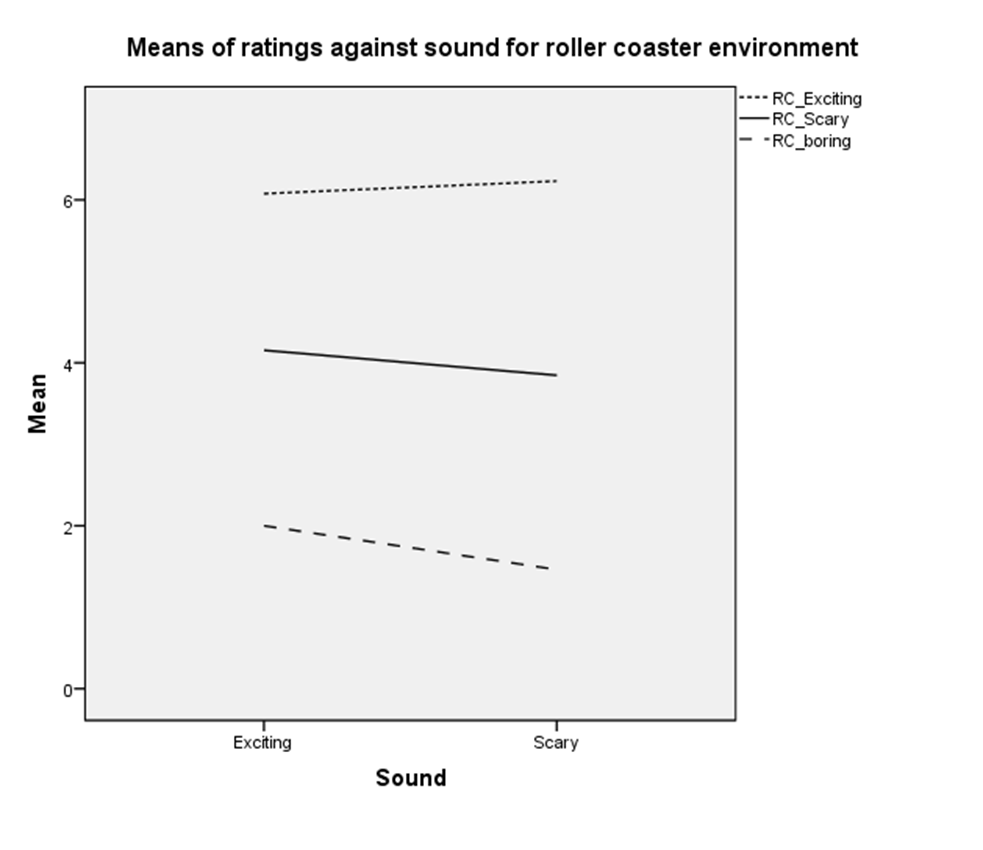
\includegraphics[width=0.90\textwidth]{Section_1/Figures/Ratings_sound_RC.png}
	\caption{Means of the ratings against the sentences the participant heard for the roller coaster environment}
	\label{fig:Ratings_sound_RC}
\end{figure}

From the figure we conclude that the participants that heard scary sentences (M= 1.46, SD = .877) not had significantly (t(24) = -1.46, p = 0.157) different ratings for boring than participants that heard the exciting sentences (M=2.00, SD = .277). Also the rating for scary was not significantly (t(24) = -.437, p= .666) different for scary sentences (M=3.85, SD=1.725) than for exciting sentences (M=4.15, SD=1.864). At last, also the rating for exciting did not have a significant difference (t(24)=.463, SD=.648) for scary sentences (M=6.23, SD =.725) than for exciting sentences (M=6.08, SD=.954). From these results we cannot conclude at this point that the sentences had an impact on the perception of the participants. \\

To check for the other ratings of the participants for the roller coaster environment, the ratings for both the exciting sentences and the scary sentences are shown in figure \ref{fig:Ratings2_sound_RC}. 

\begin{figure}[H]
	\centering
		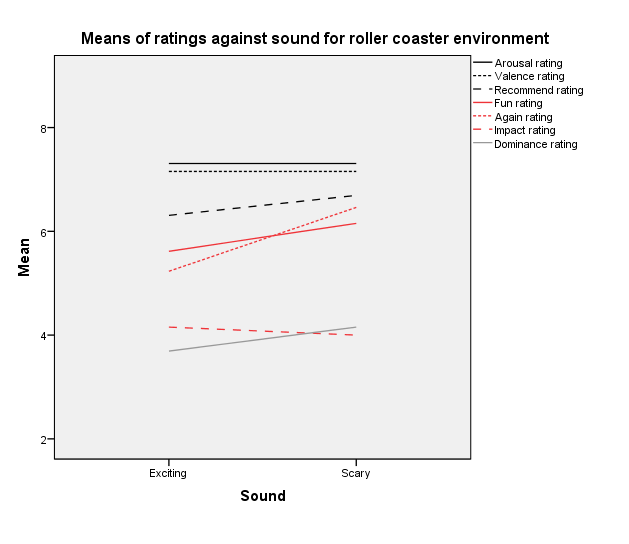
\includegraphics[width=0.90\textwidth]{Section_1/Figures/Ratings2_sound_RC.png}
	\caption{Means of the other ratings against the sentences the participant heard for the roller coaster environment}
	\label{fig:Ratings2_sound_RC}
\end{figure}

From the figure we can conclude that the biggest differences are for the ratings for again and fun, this is confirmed by performing a t-test. The rating of fun does not have a significant (t(24) = 1.351, p=.189) difference after hearing the exciting sentences (M=5.62, SD=1.121) rather than for hearing the scary sentences (M=6.15, SD=.899). However, there is a significant difference (t(24)=2.509, p=.019) for the rating of again, there is a significant difference between hearing the exciting sentences (M=5.23, SD=1.589) and hearing the scary sentences (M=6.46, SD=.776). \\

The difference why participants want to do the roller coaster experience again more when they heard the scary sentences than when they heard the exciting voices is not obvious. In the next paragraph we will try to find a reason for this. 

\section{Discussion}
For finding the reason that the results were counter intuitive for the roller coaster environment, we needed more knowledge then provided in the ratings. In the questionnaires the participants were allowed to leave comments about the voices. Especially for the roller coaster environment, the emotions of the sounds did not always seem to fit so well in the roller coaster environment. Two examples of comments are:”, “In the roller coaster ride I did not feel the same way as what the voice overs said” and “Especially during the Roller coaster ride I was much more focused on the surroundings than on the voice-overs”. The influence of the type of sentences the participants heard will be investigated now. \\

The rate in which people felt present in the environment shown against the sentence heard in the roller coaster environment is shown below. The different variables shown in figure \ref{fig:Ratings_presence_RC} are respectively: 

\begin{itemize}
	\item The sense of being in the environment;
  \item How real the virtual world seemed to them;
  \item How much the virtual environment seemed consistent to the real world experience;
  \item How aware they were of the real world surrounding while navigating in the virtual world.
\end{itemize}

\begin{figure}[H]
	\centering
		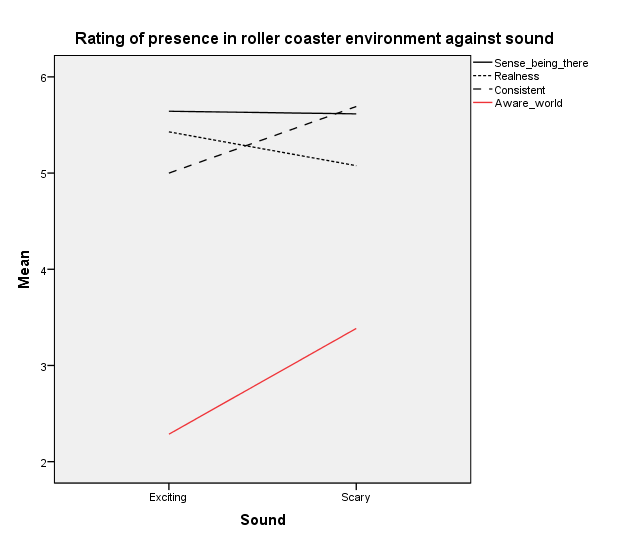
\includegraphics[width=0.90\textwidth]{Section_1/Figures/Ratings_presence_RC.png}
	\caption{The rating of the experienced presence in the roller coaster environment against the sentences the participant heard}
	\label{fig:Ratings_presence_RC}
\end{figure}

The figure shows the biggest difference for the rating of the participant to be aware about the real world while navigating in the virtual world. The results of the t-test shows that the difference after hearing the exciting sentences (M=2.29, SD=1.204) or hearing the scary sentences (M=3.38, SD=1.895) cannot be assumed to be significant (t(25) = -1.813, p = 0.082). However, the chance of 0.082 is not completely neglectable and we assume that the kind of emotion as such had a certain impact on the perception of the participants. We will compare these results with the results for the space environment, shown in figure \ref{fig:Ratings_presence_BM}.

\begin{figure}[H]
	\centering
		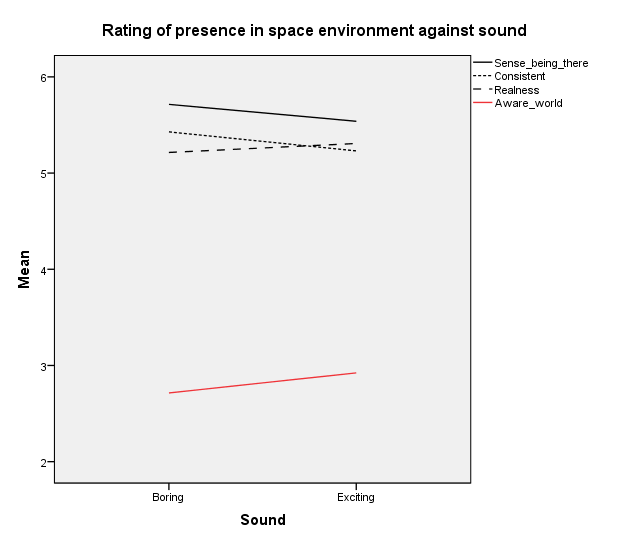
\includegraphics[width=0.90\textwidth]{Section_1/Figures/Ratings_presence_BM.png}
	\caption{The rating of the experienced presence in the space environment against the sentences the participant heard}
	\label{fig:Ratings_presence_BM}
\end{figure}

The biggest difference for a variable within the space environment is the difference in the rating for the sense of being there after hearing the boring sentences (M=5.71, SD=.726) or the exciting sentences (M=5.54, SD=1.266), however this is not a significant difference (t(25)=-.447, p=.659).\\

From this comparison, we conclude that the participants were less engaged in the roller coaster environment when they heard the exciting sentences. The emotions with which the participant’s recorded the voices for the roller coaster environment may not have fit the real emotions during the environment, and therefore might have been less convincing or maybe not convincing at all for the participants. According to the theory, a message is more convincing when it is more close to the opinion of the receiver, While the message may not be convincing, this could be the reason of the counter-intuitive result. \\

To investigate another possible cause of the result, we investigated the relation between the order in which the participants saw the environments and the ratings of the participants. It turned out that the ratings which the participants did with the Self Assessment Mannequin were the most influenced factors, at most for the rating of arousal in the space environment. This rating turned out to be lower (M=3.08, SD=1.782) when the space environment was shown first rather than the roller coaster environment (M=4.50, SD=2.210), however the difference was not significant (t(24)=1.778, p=0.088). 

\section{Combining results}
While there were positive and negative measures in the questionnaires, we checked for correlations between different answers to positive questions. To evaluate results, we first categorized the results of the questionnaires into the answers about an environment where people heard positive respectively negative sentences. The environment itself will now be ignored. 

To check for correlations in each category, we used the crombach's alpha test to check for sufficient correlation. The positive sub scale consisted of 7 items ($\alpha$ = .857) and the same items were chosen on purpose for the negative sub scale ($\alpha$ = .729) to have the same way of computing the positivity measure. These items were: 
\begin{itemize}
	\item Exciting;
	\item Again;
	\item Fun;
	\item Recommend;
	\item Impact;
	\item Valence;
	\item The inverse value of boring.
\end{itemize}

The answers about how scary the environment was were not used in the sub scales. The reason is that scary was strongly correlating with for example exciting (r(26) = .516, p=0.007), the inverse of boring, (r(26)=.776, p $<$ 0.00) and fun (r(26) = .526, p = 0.006). However, we assumed scary to be negative and now it is positively correlated with positive measures. Therefore the results of scary were not used. The 7 items are combined in one measure, positivity, which represents how positive the emotion of the participant is about the experience.

The results of the t-test, comparing the combined measure positivity, showed that the difference between positive (M=4.71, SD=1.346) and negative (M=4.68, SD=1.474) stimuli was not significant (t(50)=0.094, p=.925). As a reference, the results where scary was considered showed more difference but still not a significant (t(50)=1.948), p = 0.057) difference between the ratings after positive stimuli (M=4.86, SD=1.180) and negative stimuli (M=4.23, p = 1.158).

The two figures below show the boxplots of the positivity, the first without considering scary and the second, as a comparison, with scary.

\begin{figure}[H]
	\centering
		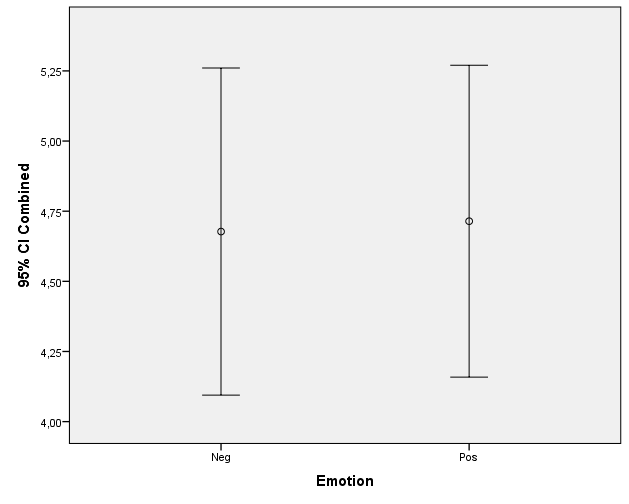
\includegraphics[width=0.70\textwidth]{Section_1/Figures/Boxplot_emo1.png}
	\caption{The combined rating of the positivity of the participant against the received stimuli}
	\label{fig:Boxplot_combined}
\end{figure}	

\begin{figure}[H]
	\centering
		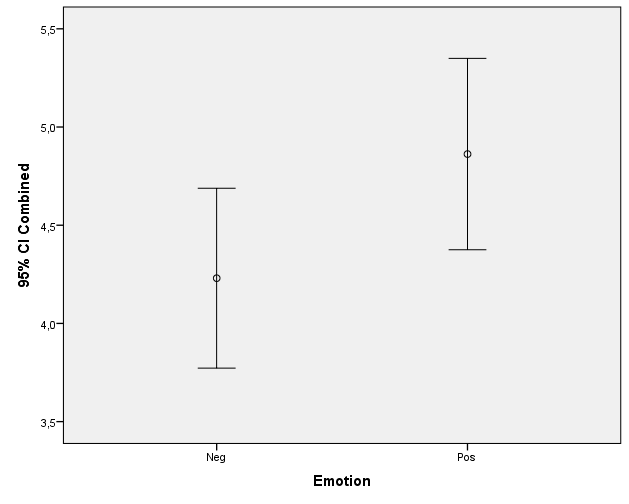
\includegraphics[width=0.70\textwidth]{Section_1/Figures/Boxplot_emo2.png}
	\caption{The combined rating of the positivity of the participant including the rating for scary against the received stimuli}
	\label{fig:Boxplot_combined2}
\end{figure}	

In the boxplots can be seen that without considering scary there is not much difference between the ratings. The results including scary show a lot more difference, however in a counter-intuitive way. From this we conclude that scary might not be a representative negative emotion opposing to the positive emotion exciting for the roller coaster environment.

\subsection{Within-subject analysis}
In the investigation there were only 13 usable results to perform a within-subjects analysis between subjects that heard positive and negative sentences. The results didn't show a significant difference in rating of the environment after hearing positive or negative sentences, so we will not go into details. More participants hearing one positive and one negative stimulus were needed to yield results for a within-subject analysis. 
 
\end{document}